\documentclass[../main.tex]{subfiles}

\begin{document}
\section{Results}
\subsection{Classification}
\subsubsection{Logistic regression}


\begin{figure}[H] 
   \centering
   \begin{subfigure}[b]{0.45\textwidth}
      \centering
    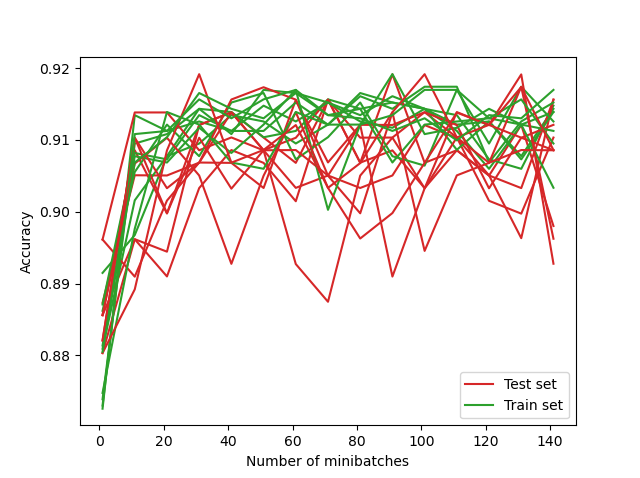
\includegraphics[width=\textwidth]{../assets/acc_vs_mb_set_40.png}
    \caption{}
    \label{fig:accvsepoch}
   \end{subfigure}
   \quad
   \begin{subfigure}[b]{0.45\textwidth}
    \centering
    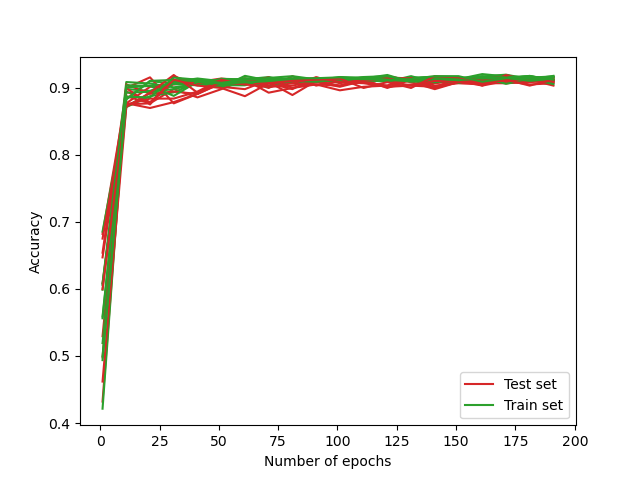
\includegraphics[width=\textwidth]{../assets/acc_vs_epoch_set_110.png} 
    \caption{}
    \label{fig:accvsmini}
   \end{subfigure}
   \caption{(a) Plot of the accuracy vs. the number of epochs in logistic regression with constant epoch=110 (b) Plot of the accuracy vs. the number of minibatches in logistic regression with constant minibatch=40
   }
   \label{fig:terrain-OLS}
\end{figure} 


\subsubsection{Neural network for classification}

\subsection{Regression}
\end{document}